
\documentclass[11pt]{article}
\usepackage{times}
\usepackage{url}
\usepackage{latexsym}
\usepackage[utf8]{inputenc}  %% to get umlauts right
\usepackage{graphicx}
\usepackage{covington}

\usepackage{breakcites}
 
\setlength{\topmargin}{-1cm}
\setlength{\textheight}{23cm}
\setlength{\oddsidemargin}{0.0cm}
\setlength{\textwidth}{16cm}


\pagestyle{myheadings}    % Go for customized headings
\markboth{Test}{MyName: MyProjectTitle \hspace{2cm} \today \hfill }


\begin{document}


\begin{titlepage}

\includegraphics[height=20mm]{uzh_logo_d_pos}\\

\begin{center}

{\sffamily
Seminar \\
\textbf{Fortgeschrittene Techniken der Maschinellen Übersetzung} \\
Herbstsemester 2014 \\

\vspace{2cm}

{\Huge (Titel)}\\

\vspace{4cm}

\textbf{Verfasserin/Verfasser: (Vorname Name)} \\
	Matrikel-Nr: (xx-xxx-xxx) \\

\vspace{2cm}

Dozenten: Mark Fishel, Martin Volk

% Assistent: Johannes Graën

Institut f\"ur Computerlinguistik

\vfill Abgabedatum: (xx.xx.xxxx) 

\vspace{3cm}
}
\end{center}

\end{titlepage}

\newpage



% \begin{abstract}
% The abstract goes here, if you want to use it. It is optional ...
% \end{abstract}


\section{Introduction}

Your motivation for the topic should go here and your main research questions. 

The document structure is just an example. You may structure your document differently. You may write in English or German. Your seminar paper should have around 15 pages.

\section{Background - Please find good chapter headings!}

A summary of related research should go here. It can be structured with subsections.

\subsection{Parallel Corpora for SMT}

\subsection{Parallel Corpora for Linguistics}

\section{Experiments}

A description of your work should go here.

You should cite a book or a paper with author name and year. Examples: with 1 author \cite{Koehn2005}, with 2 authors \cite{Jurafsky2009}, and with 3 or more authors \cite{Masc2014}.

Here is also an example of how you can include an image (see the Kokos screen in figure \ref{Kokos_screen}).

\section{Conclusion}

A summary of your main findings goes here. Please also mention open research issues.



\begin{figure*}
\begin{center}
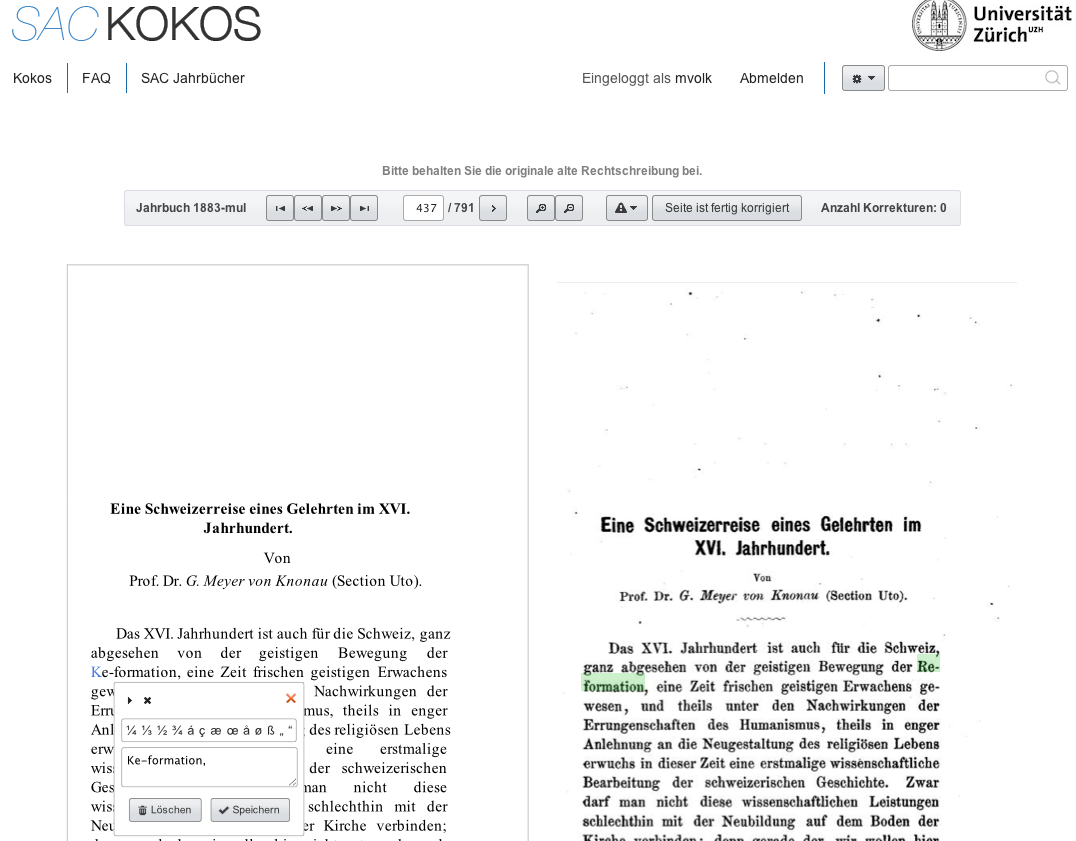
\includegraphics[height=9.5cm]{Kokos_Screen_Shot.png}
\end{center}
\caption{Example of a Screenshot} \label{Kokos_screen}
\end{figure*}

 


\bibliographystyle{apalike}
% your bib file should go here 
\bibliography{Volk_example_bibfile}



\end{document}
